\documentclass[a4paper,twocolumn]{article}

\usepackage[english]{babel}
\usepackage[utf8]{inputenc}
\usepackage{graphicx}
\usepackage{fullpage}

\usepackage{titlesec}

\titleformat*{\section}{\large\bfseries}
\titleformat*{\subsection}{\normalsize\bfseries}


\title{Distilling the Knowledge in a Neural Network $-$ summary}
\author{Matěj Nikl}

\begin{document}
\maketitle
A process called \textit{distillation} is a kind of learning that can be used to transfer a knowledge from a cumbersome model (or an ensemble of models) to a smaller/single model, which is more suitable for deployment, while preserving the knowledge and thus preserving the performance.

To do so, the standard back-propagation algorithm (with a different objective function) is used.

\section{Softmax with temperature}
Neural networks typically produce class probabilities by using a \textit{softmax} output layer that converts the logit, $z_i$, computed for each class into a probability, $q_i$, by comparing $z_i$ with the other logits
\[
    q_i = \frac{e^{z_i/T}}{\sum_j e^{z_j/T}}
\]
where a temperature $T$ is normally set to 1. Using a higher value for $T$ produces a softer probability distribution over classes.

\begin{figure}[!h]
    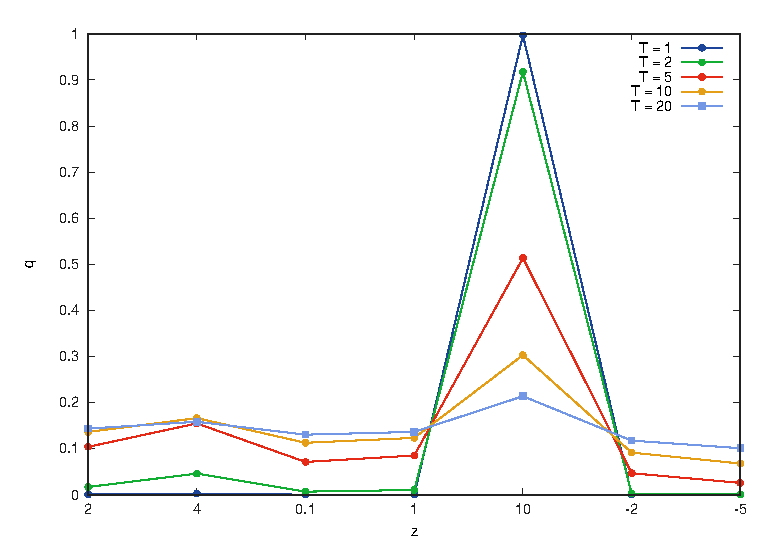
\includegraphics[width=\columnwidth]{softmax_example.eps}
    \caption{Comparison of softmax outputs $q$ given inputs $z$ using different temperatures}
\end{figure}

\section{Distillation}

A side-effect of learning is that a trained model assigns probabilities to all of the incorrect answers and even when these probabilities are very small, some of them are much larger than others $-$ the relative probabilities of incorrect answers tell us a lot about how the model tends to generalize. An image of a car, for example, may only have a very small chance of being mistaken for a truck, but that mistake is still much more probable than mistaking it for an apple.

By using all the class probabilities produced by a cumbersome model as \textit{soft targets} for a small model, the knowledge can be transferred.

For this transfer stage, the same training set or even a different \textit{transfer} set can be used.

For an ensemble of models, an arithmetic or geometric mean of their individual predictive distributions as the soft targets can be used.

Moreover, when the soft targets have high entropy, they provide much more information per training case than hard targets and much less variance in the gradient between training cases, so the small model can often be trained on much less data and using a much higher learning rate.

\begin{table*}[t]
    \center
    \begin{tabular}{| c | c | c |}
        \hline
        System                 & Test Frame Accuracy & WER    \\ \hline
        Baseline               & 58.9\%              & 10.9\% \\
        10x Ensemble           & 61.1\%              & 10.7\% \\
        Distilled single model & 60.8\%              & 10.7\% \\
        \hline
    \end{tabular}
    \caption{Frame classification accuracy and Word Error Rate (WER) of a speech recognition DNN showing that the distilled single model performs about as well as the averaged prediction of 10 models that were used to create the soft targets.}
\end{table*}

\begin{table*}[t]
    \center
    \begin{tabular}{| l | c | c |}
        \hline
        System \& training set             & Train Frame Accuracy & Test Frame Accuracy \\ \hline
        Baseline (100\% of training set)   & 63.4\%               & 58.9\%              \\
        Baseline (3\% of training set)     & 67.3\%               & 44.5\%              \\
        Soft Targets (3\% of training set) & 65.4\%               & 57.0\%              \\
        \hline
    \end{tabular}
    \caption{Soft targets allow a new model to generalize well from only 3\% of the training set. The soft targets are obtained by training on the full training set.}
\end{table*}


\subsection{Computing the gradient}
Using the Kullback-Leibler divergence as a loss function:
\[
    C = - \sum_i p_i log(q_i)
\]
Each case in the transfer set contributes a cross-entropy gradient, $dC/dz_i$, with respect to each logit, $z_i$, of the distilled model. If the cumbersome model has logits $v_i$, which produce soft target probabilities $p_i$ and the transfer training is done at a temperature of $T$, this gradient is given by:
\[
    \frac{\partial C}{\partial z_i} = \frac{1}{T}(q_i - p_i) = \frac{1}{T}\left( \frac{e^{z_i/T}}{\sum_j e^{z_j/T}} - \frac{e^{v_i/T}}{\sum_j e^{v_j/T}} \right)
\]
If the temperature is high compared with the magnitude of the logits, we can approximate ($e^x \approx 1+x$ for $x \approx 0$):
\[
    \frac{\partial C}{\partial z_i} \approx \frac{1}{T}\left( \frac{1 + z_i/T}{N + \sum_j z_j/T} - \frac{1 + v_i/T}{N + \sum_j v_j/T} \right)
\]
If we now assume that the logits have been zero-meaned separately for each transfer case so that $\sum_j z_j = \sum_j v_j = 0$, we can further simplify to:
\[
    \frac{\partial C}{\partial z_i} \approx \frac{1}{NT^2} (z_i - v_i)
\]
So in the high temperature limit, distillation is equivalent to minimizing the L2 distance (MSE) between the soft target probabilities and the distilled model probabilities.

\subsection{Combining the objective functions}
When the correct labels are known for all or at least some of the transfer set, this method can be significantly improved by also training the distilled model to produce the correct labels. The best way to do it is to use a weighted average of the above defined objective function of cross-entropy with the soft targets and the objective function of cross-entropy with the correct labels (the hard targets). The best results are generally obtained by using a \textit{considerably} lower weight on the second objective function.

\section{Ensembles of specialists on very big datasets}
Even though training an ensemble of models is a very simple way to take advantage of parallel computation, and distillation can help us at the test time, the amount of computation required at training time for a very large dataset is excessive.

The proposed improvement for this situation is, instead of training an ensemble of standalone models, to train \textit{specialist} models that can help with distinguishing between highly confusable classes, while improving the overall performance.

Each specialist model starts with weights initialized as the main \textit{generalist} model and focuses solely on its own subset of (for the generalist model) highly confusable classes, and thus learns much faster.

The ultimate goal of this idea was to distill the knowledge from the specialist models back into the generalist model, which the researchers haven't yet been able to accomplish.

\end{document}
